
%% bare_conf.tex
%% V1.3
%% 2007/01/11
%% by Michael Shell
%% See:
%% http://www.michaelshell.org/
%% for current contact information.
%%
%% This is a skeleton file demonstrating the use of IEEEtran.cls
%% (requires IEEEtran.cls version 1.7 or later) with an IEEE conference paper.
%%
%% Support sites:
%% http://www.michaelshell.org/tex/ieeetran/
%% http://www.ctan.org/tex-archive/macros/latex/contrib/IEEEtran/
%% and
%% http://www.ieee.org/

%%*************************************************************************
%% Legal Notice:
%% This code is offered as-is without any warranty either expressed or
%% implied; without even the implied warranty of MERCHANTABILITY or
%% FITNESS FOR A PARTICULAR PURPOSE! 
%% User assumes all risk.
%% In no event shall IEEE or any contributor to this code be liable for
%% any damages or losses, including, but not limited to, incidental,
%% consequential, or any other damages, resulting from the use or misuse
%% of any information contained here.
%%
%% All comments are the opinions of their respective authors and are not
%% necessarily endorsed by the IEEE.
%%
%% This work is distributed under the LaTeX Project Public License (LPPL)
%% ( http://www.latex-project.org/ ) version 1.3, and may be freely used,
%% distributed and modified. A copy of the LPPL, version 1.3, is included
%% in the base LaTeX documentation of all distributions of LaTeX released
%% 2003/12/01 or later.
%% Retain all contribution notices and credits.
%% ** Modified files should be clearly indicated as such, including  **
%% ** renaming them and changing author support contact information. **
%%
%% File list of work: IEEEtran.cls, IEEEtran_HOWTO.pdf, bare_adv.tex,
%%                    bare_conf.tex, bare_jrnl.tex, bare_jrnl_compsoc.tex
%%*************************************************************************

% *** Authors should verify (and, if needed, correct) their LaTeX system  ***
% *** with the testflow diagnostic prior to trusting their LaTeX platform ***
% *** with production work. IEEE's font choices can trigger bugs that do  ***
% *** not appear when using other class files.                            ***
% The testflow support page is at:
% http://www.michaelshell.org/tex/testflow/



% Note that the a4paper option is mainly intended so that authors in
% countries using A4 can easily print to A4 and see how their papers will
% look in print - the typesetting of the document will not typically be
% affected with changes in paper size (but the bottom and side margins will).
% Use the testflow package mentioned above to verify correct handling of
% both paper sizes by the user's LaTeX system.
%
% Also note that the "draftcls" or "draftclsnofoot", not "draft", option
% should be used if it is desired that the figures are to be displayed in
% draft mode.
%
\documentclass[10pt, conference, compsocconf]{IEEEtran}
% Add the compsocconf option for Computer Society conferences.
%
% If IEEEtran.cls has not been installed into the LaTeX system files,
% manually specify the path to it like:
% \documentclass[conference]{../sty/IEEEtran}





% Some very useful LaTeX packages include:
% (uncomment the ones you want to load)


% *** MISC UTILITY PACKAGES ***
%
%\usepackage{ifpdf}
% Heiko Oberdiek's ifpdf.sty is very useful if you need conditional
% compilation based on whether the output is pdf or dvi.
% usage:
% \ifpdf
%   % pdf code
% \else
%   % dvi code
% \fi
% The latest version of ifpdf.sty can be obtained from:
% http://www.ctan.org/tex-archive/macros/latex/contrib/oberdiek/
% Also, note that IEEEtran.cls V1.7 and later provides a builtin
% \ifCLASSINFOpdf conditional that works the same way.
% When switching from latex to pdflatex and vice-versa, the compiler may
% have to be run twice to clear warning/error messages.






% *** CITATION PACKAGES ***
%
%\usepackage{cite}
% cite.sty was written by Donald Arseneau
% V1.6 and later of IEEEtran pre-defines the format of the cite.sty package
% \cite{} output to follow that of IEEE. Loading the cite package will
% result in citation numbers being automatically sorted and properly
% "compressed/ranged". e.g., [1], [9], [2], [7], [5], [6] without using
% cite.sty will become [1], [2], [5]--[7], [9] using cite.sty. cite.sty's
% \cite will automatically add leading space, if needed. Use cite.sty's
% noadjust option (cite.sty V3.8 and later) if you want to turn this off.
% cite.sty is already installed on most LaTeX systems. Be sure and use
% version 4.0 (2003-05-27) and later if using hyperref.sty. cite.sty does
% not currently provide for hyperlinked citations.
% The latest version can be obtained at:
% http://www.ctan.org/tex-archive/macros/latex/contrib/cite/
% The documentation is contained in the cite.sty file itself.






% *** GRAPHICS RELATED PACKAGES ***
%
\ifCLASSINFOpdf
  % \usepackage[pdftex]{graphicx}
  % declare the path(s) where your graphic files are
  % \graphicspath{{../pdf/}{../jpeg/}}
  % and their extensions so you won't have to specify these with
  % every instance of \includegraphics
  % \DeclareGraphicsExtensions{.pdf,.jpeg,.png}
\else
  % or other class option (dvipsone, dvipdf, if not using dvips). graphicx
  % will default to the driver specified in the system graphics.cfg if no
  % driver is specified.
  % \usepackage[dvips]{graphicx}
  % declare the path(s) where your graphic files are
  % \graphicspath{{../eps/}}
  % and their extensions so you won't have to specify these with
  % every instance of \includegraphics
  % \DeclareGraphicsExtensions{.eps}
\fi
% graphicx was written by David Carlisle and Sebastian Rahtz. It is
% required if you want graphics, photos, etc. graphicx.sty is already
% installed on most LaTeX systems. The latest version and documentation can
% be obtained at: 
% http://www.ctan.org/tex-archive/macros/latex/required/graphics/
% Another good source of documentation is "Using Imported Graphics in
% LaTeX2e" by Keith Reckdahl which can be found as epslatex.ps or
% epslatex.pdf at: http://www.ctan.org/tex-archive/info/
%
% latex, and pdflatex in dvi mode, support graphics in encapsulated
% postscript (.eps) format. pdflatex in pdf mode supports graphics
% in .pdf, .jpeg, .png and .mps (metapost) formats. Users should ensure
% that all non-photo figures use a vector format (.eps, .pdf, .mps) and
% not a bitmapped formats (.jpeg, .png). IEEE frowns on bitmapped formats
% which can result in "jaggedy"/blurry rendering of lines and letters as
% well as large increases in file sizes.
%
% You can find documentation about the pdfTeX application at:
% http://www.tug.org/applications/pdftex





% *** MATH PACKAGES ***
%
%\usepackage[cmex10]{amsmath}
% A popular package from the American Mathematical Society that provides
% many useful and powerful commands for dealing with mathematics. If using
% it, be sure to load this package with the cmex10 option to ensure that
% only type 1 fonts will utilized at all point sizes. Without this option,
% it is possible that some math symbols, particularly those within
% footnotes, will be rendered in bitmap form which will result in a
% document that can not be IEEE Xplore compliant!
%
% Also, note that the amsmath package sets \interdisplaylinepenalty to 10000
% thus preventing page breaks from occurring within multiline equations. Use:
%\interdisplaylinepenalty=2500
% after loading amsmath to restore such page breaks as IEEEtran.cls normally
% does. amsmath.sty is already installed on most LaTeX systems. The latest
% version and documentation can be obtained at:
% http://www.ctan.org/tex-archive/macros/latex/required/amslatex/math/





% *** SPECIALIZED LIST PACKAGES ***
%
%\usepackage{algorithmic}
% algorithmic.sty was written by Peter Williams and Rogerio Brito.
% This package provides an algorithmic environment fo describing algorithms.
% You can use the algorithmic environment in-text or within a figure
% environment to provide for a floating algorithm. Do NOT use the algorithm
% floating environment provided by algorithm.sty (by the same authors) or
% algorithm2e.sty (by Christophe Fiorio) as IEEE does not use dedicated
% algorithm float types and packages that provide these will not provide
% correct IEEE style captions. The latest version and documentation of
% algorithmic.sty can be obtained at:
% http://www.ctan.org/tex-archive/macros/latex/contrib/algorithms/
% There is also a support site at:
% http://algorithms.berlios.de/index.html
% Also of interest may be the (relatively newer and more customizable)
% algorithmicx.sty package by Szasz Janos:
% http://www.ctan.org/tex-archive/macros/latex/contrib/algorithmicx/




% *** ALIGNMENT PACKAGES ***
%
%\usepackage{array}
% Frank Mittelbach's and David Carlisle's array.sty patches and improves
% the standard LaTeX2e array and tabular environments to provide better
% appearance and additional user controls. As the default LaTeX2e table
% generation code is lacking to the point of almost being broken with
% respect to the quality of the end results, all users are strongly
% advised to use an enhanced (at the very least that provided by array.sty)
% set of table tools. array.sty is already installed on most systems. The
% latest version and documentation can be obtained at:
% http://www.ctan.org/tex-archive/macros/latex/required/tools/


%\usepackage{mdwmath}
%\usepackage{mdwtab}
% Also highly recommended is Mark Wooding's extremely powerful MDW tools,
% especially mdwmath.sty and mdwtab.sty which are used to format equations
% and tables, respectively. The MDWtools set is already installed on most
% LaTeX systems. The lastest version and documentation is available at:
% http://www.ctan.org/tex-archive/macros/latex/contrib/mdwtools/


% IEEEtran contains the IEEEeqnarray family of commands that can be used to
% generate multiline equations as well as matrices, tables, etc., of high
% quality.


%\usepackage{eqparbox}
% Also of notable interest is Scott Pakin's eqparbox package for creating
% (automatically sized) equal width boxes - aka "natural width parboxes".
% Available at:
% http://www.ctan.org/tex-archive/macros/latex/contrib/eqparbox/





% *** SUBFIGURE PACKAGES ***
%\usepackage[tight,footnotesize]{subfigure}
% subfigure.sty was written by Steven Douglas Cochran. This package makes it
% easy to put subfigures in your figures. e.g., "Figure 1a and 1b". For IEEE
% work, it is a good idea to load it with the tight package option to reduce
% the amount of white space around the subfigures. subfigure.sty is already
% installed on most LaTeX systems. The latest version and documentation can
% be obtained at:
% http://www.ctan.org/tex-archive/obsolete/macros/latex/contrib/subfigure/
% subfigure.sty has been superceeded by subfig.sty.



%\usepackage[caption=false]{caption}
%\usepackage[font=footnotesize]{subfig}
% subfig.sty, also written by Steven Douglas Cochran, is the modern
% replacement for subfigure.sty. However, subfig.sty requires and
% automatically loads Axel Sommerfeldt's caption.sty which will override
% IEEEtran.cls handling of captions and this will result in nonIEEE style
% figure/table captions. To prevent this problem, be sure and preload
% caption.sty with its "caption=false" package option. This is will preserve
% IEEEtran.cls handing of captions. Version 1.3 (2005/06/28) and later 
% (recommended due to many improvements over 1.2) of subfig.sty supports
% the caption=false option directly:
%\usepackage[caption=false,font=footnotesize]{subfig}
%
% The latest version and documentation can be obtained at:
% http://www.ctan.org/tex-archive/macros/latex/contrib/subfig/
% The latest version and documentation of caption.sty can be obtained at:
% http://www.ctan.org/tex-archive/macros/latex/contrib/caption/




% *** FLOAT PACKAGES ***
%
%\usepackage{fixltx2e}
% fixltx2e, the successor to the earlier fix2col.sty, was written by
% Frank Mittelbach and David Carlisle. This package corrects a few problems
% in the LaTeX2e kernel, the most notable of which is that in current
% LaTeX2e releases, the ordering of single and double column floats is not
% guaranteed to be preserved. Thus, an unpatched LaTeX2e can allow a
% single column figure to be placed prior to an earlier double column
% figure. The latest version and documentation can be found at:
% http://www.ctan.org/tex-archive/macros/latex/base/



%\usepackage{stfloats}
% stfloats.sty was written by Sigitas Tolusis. This package gives LaTeX2e
% the ability to do double column floats at the bottom of the page as well
% as the top. (e.g., "\begin{figure*}[!b]" is not normally possible in
% LaTeX2e). It also provides a command:
%\fnbelowfloat
% to enable the placement of footnotes below bottom floats (the standard
% LaTeX2e kernel puts them above bottom floats). This is an invasive package
% which rewrites many portions of the LaTeX2e float routines. It may not work
% with other packages that modify the LaTeX2e float routines. The latest
% version and documentation can be obtained at:
% http://www.ctan.org/tex-archive/macros/latex/contrib/sttools/
% Documentation is contained in the stfloats.sty comments as well as in the
% presfull.pdf file. Do not use the stfloats baselinefloat ability as IEEE
% does not allow \baselineskip to stretch. Authors submitting work to the
% IEEE should note that IEEE rarely uses double column equations and
% that authors should try to avoid such use. Do not be tempted to use the
% cuted.sty or midfloat.sty packages (also by Sigitas Tolusis) as IEEE does
% not format its papers in such ways.





% *** PDF, URL AND HYPERLINK PACKAGES ***
%
%\usepackage{url}
% url.sty was written by Donald Arseneau. It provides better support for
% handling and breaking URLs. url.sty is already installed on most LaTeX
% systems. The latest version can be obtained at:
% http://www.ctan.org/tex-archive/macros/latex/contrib/misc/
% Read the url.sty source comments for usage information. Basically,
% \url{my_url_here}.





% *** Do not adjust lengths that control margins, column widths, etc. ***
% *** Do not use packages that alter fonts (such as pslatex).         ***
% There should be no need to do such things with IEEEtran.cls V1.6 and later.
% (Unless specifically asked to do so by the journal or conference you plan
% to submit to, of course. )


% correct bad hyphenation here
\hyphenation{op-tical net-works semi-conduc-tor}

% provided by users
\usepackage{psfrag}
\usepackage{amssymb}
%\usepackage{theorem}
\def\comment#1{}
\usepackage{fancyvrb}
\usepackage{alltt}
\usepackage{listings}
\usepackage{url}
\usepackage[linesnumbered]{algorithm2e}
%\usepackage{program}
%\usepackage{array}
\usepackage{hyperref}
%\usepackage{microtype}
%\usepackage{algorithm}
%\usepackage{algorithmic}

%\def\IEEEbibitemsep{2pt plus .5pt}
\IEEEoverridecommandlockouts


\begin{document}
%
% paper title
% can use linebreaks \\ within to get better formatting as desired
\title{Formal Specification and Model Checking \\the Abstract Autonomous Vehicle
Merging Point Protocol
%\thanks{This work was partially supported by }
%\thanks{DOI reference number: 10.18293/DMSVIVA2021-004 }
}

% author names and affiliations
% use a multiple column layout for up to two different
% affiliations

\author{\IEEEauthorblockN{Liu Minxuan, Dang Duy Bui, Duong Dinh Tran, Kazuhiro Ogata}
\IEEEauthorblockA{School of Information Science\\
Japan Advanced Institute of Science and Technology (JAIST)\\
1-1 Asahidai, Nomi, Ishikawa 923-1292, Japan\\
Email: \{liuminxuan,bddang,duongtd,ogata\}@jaist.ac.jp}
}

%\author{\IEEEauthorblockN{Authors Name/s per 1st Affiliation (Author)}
%\IEEEauthorblockA{line 1 (of Affiliation): dept. name of organization\\
%line 2: name of organization, acronyms acceptable\\
%line 3: City, Country\\
%line 4: Email: name@xyz.com}
%\and
%\IEEEauthorblockN{Authors Name/s per 2nd Affiliation (Author)}
%\IEEEauthorblockA{line 1 (of Affiliation): dept. name of organization\\
%line 2: name of organization, acronyms acceptable\\
%line 3: City, Country\\
%line 4: Email: name@xyz.com}
%}

% conference papers do not typically use \thanks and this command
% is locked out in conference mode. If really needed, such as for
% the acknowledgment of grants, issue a \IEEEoverridecommandlockouts
% after \documentclass

% for over three affiliations, or if they all won't fit within the width
% of the page, use this alternative format:
% 
%\author{\IEEEauthorblockN{Michael Shell\IEEEauthorrefmark{1},
%Homer Simpson\IEEEauthorrefmark{2},
%James Kirk\IEEEauthorrefmark{3}, 
%Montgomery Scott\IEEEauthorrefmark{3} and
%Eldon Tyrell\IEEEauthorrefmark{4}}
%\IEEEauthorblockA{\IEEEauthorrefmark{1}School of Electrical and Computer Engineering\\
%Georgia Institute of Technology,
%Atlanta, Georgia 30332--0250\\ Email: see http://www.michaelshell.org/contact.html}
%\IEEEauthorblockA{\IEEEauthorrefmark{2}Twentieth Century Fox, Springfield, USA\\
%Email: homer@thesimpsons.com}
%\IEEEauthorblockA{\IEEEauthorrefmark{3}Starfleet Academy, San Francisco, California 96678-2391\\
%Telephone: (800) 555--1212, Fax: (888) 555--1212}
%\IEEEauthorblockA{\IEEEauthorrefmark{4}Tyrell Inc., 123 Replicant Street, Los Angeles, California 90210--4321}}




% use for special paper notices
%\IEEEspecialpapernotice{(Invited Paper)}




% make the title area
\maketitle

\begin{abstract}
Self-driving vehicles are promise transportation of the future providing many conveniences for people.
Since safety is paramount for any autonomous vehicle system, there is a large number of researches have been proposed to automatically control vehicles running on public roads without any collision.
An autonomous vehicle protocol for merge points or a merging protocol proposed  by S. Aoki and R. Rajkumar is an interaction-based traffic protocol for safely cross a merge point, which is the intersection of 2 one-way lanes merging into one lane. 
Based on that protocol, in this paper, we make some modifications by abstract some concepts.
We then formally specify the protocol in Maude, and conduct model checking to confirm that the protocol enjoys some important properties such as the non-collision property. 

%We have revised SMGA so as to handle composite data. 
%SMGA is a tool that mainly supports humans in visually perceiving the characteristics/properties of systems/protocols. Those characteristics could be used as lemmas to formally verify that the systems/protocols enjoy desired properties. The core task of the tool is to design a state picture that helps humans better understanding the systems/protocols and/or conjecturing the characteristics. 
%To demonstrate that SMGA can be applied to the wider class of systems/applications, we have graphically animated the Lim-Jeong-Park-Lee autonomous vehicle intersection control protocol with SMGA.
%The state machine formalizing the protocol uses composite data. 
%We have revised SMGA so as to handle composite data. 
%We design a flexible state picture for the protocol so that it is possible to deal with different initial states when the number of vehicles is less than or equal to a given number.
%Some characteristics are guessed by observing graphical animations based on the state picture design, and the characteristics are confirmed with model checking.
%The paper also summarizes several lessons learned as tips on how to design a state picture with composite data.

\end{abstract}

\begin{IEEEkeywords}
merging protocol; a-merging protocol; Maude; model checking

% anti-fairness; fairness; linear temporal logic; liveness property;
% model checking;
\end{IEEEkeywords}

% For peer review papers, you can put extra information on the cover
% page as needed:
% \ifCLASSOPTIONpeerreview
% \begin{center} \bfseries EDICS Category: 3-BBND \end{center}
% \fi
%
% For peerreview papers, this IEEEtran command inserts a page break and
% creates the second title. It will be ignored for other modes.
\IEEEpeerreviewmaketitle


\setlength{\parindent}{1em}
\section{Introduction}
 \label{sect_intro}
In recent years, there is a subtle amount of attention being focused on building self-driving vehicles all around the world.
In addition to the necessary hardware, the software technologies behind are considered as the key point of any self-driving system.
Any self-driving vehicle must be fully controlled so that it can not only run on the straight road but also is able to safely change to another lane, pass through an 4-way intersection, or merge lane through a merge point, just to mention a few.
Research in self-driving technology has been intensively learned, resulting in more and more safe and efficient protocols/systems dedicated to resolving such challenges.

%~\cite{10.1145/3055004.3055028} have proposed the protocol called merging protocol.
An autonomous vehicle protocol for merge points or a \textit{merging} protocol~\cite{10.1145/3055004.3055028} proposed by S. Aoki and R. Rajkumar is an interaction-based traffic protocol for safely cross a merge point, which is the intersection of 2 one-way lanes merging into one lane. 
In the protocol, self-driving vehicles are assumed to use both vehicle-to-vehicle (V2V) communications and
sensor-based perception systems.
According to the paper, the authors claimed that the protocol is safe and efficient.

In the present paper, our target aims to formally check that the merging protocol enjoys some desired properties or not. For example, we are most interested in the mutual exclusion (or non-collision) property, which says that is not more than one vehicle located at the merge point at any time.
This property is really important since if two self-driving vehicles are allowed to enter the merge point simultaneously, they will collide with each other, leading to an accident.
However, we first revise the protocol to make our version distinguish from the original \textit{merging} protocol~\cite{10.1145/3055004.3055028} by abstract some concepts.
For example, we use semaphore instead of using sending or receiving messages to control self-driving vehicles. 
We also allow vehicles to make a query to the controller of the merge point at any time.
Then, we formally specify the protocol in Maude~\cite{Clavel2007LNCS}, a rewriting logic-based specification/programming, and conduct model checking to confirm that whether the protocol enjoys our desired properties.
The experiment with six vehicles participating shows that the protocol enjoys the mutual exclusion property.

The rest of this paper is organized as follows. Sect.\,\ref{sect_Prel}
mentions some preliminaries such as state machines, and Maude.
Sect.\,\ref{sect_oriproto} introduces the \textit{merging} protocol.
Sect.\,\ref{sect_reviproto} describes our revised version of the protocol.
In Sect.\,\ref{sect_formal}, we specify our proposed protocol in Maude and model check some properties in Sect.\,\ref{sect_model}.
Sect.\,\ref{sect_Relate} mentions some related work.
Finally, we conclude the present paper in Sect.\,\ref{concl_sect}.

The specification of the protocol in Maude presented in this
paper is available at \url{http://}.


\section{Preliminaries}
 \label{sect_Prel}
 
 
A Kripke structure $K$ is $\langle S,I,T,P,L \rangle$, where $S$ is a set
of states, $I \subseteq S$ is the set of initial states, $T \subseteq S \times S$
is a total binary relation over $S$, $P$ is a set of atomic
propositions and $L$ is a labeling function whose type is
$S \rightarrow 2^P$ . Each element $(s, s') \in T$ is called a state transition
from $s$ to $s'$ and $T$ may be called the state transitions
(with respect to $K$). For a state $s \in S$, $L(s)$ is the set
of atomic propositions that hold in $s$. A path $\pi$ is an infinite
sequence $s_0, \ldots , s_i, s_{i+1}, \ldots$ of states such that $s_i \in S$ and
$(s_i, s_{i+1}) \in T$ for each $i$. Let $\pi^i$ be $s_i, s_{i+1}, \ldots$ and $\pi(i)$ be
$s_i$. Let $P$ be the set of all paths. $\pi$ is called a computation
if $\pi(0) \in I$. Let $C$ be the set of all computations.

The syntax of a formula $\varphi$ in LTL for $K$ is $\varphi ::= \top \:|\: p \:|\: \neg \varphi \:|\: \varphi \land \varphi \:|\: \bigcirc \varphi \:|\: \varphi \: \mathcal{U} \: \varphi$, where $p \in P$. 
Let $\cal F$ be the set of all formulas in LTL for $K$. 
An arbitrary path $\pi \in P$ of $K$ and an arbitrary LTL formula $\varphi \in \cal F$ of $K$,
$K, \pi \models \varphi$ is inductively defined as $K, \pi \models \top$, $K, \pi \models p$ iff
$p \in L(\pi(0))$, $K, \pi \models \neg \varphi_1$ iff $K, \pi \not\models \varphi_1$, 
$K, \pi \models \varphi_1 \land \varphi_2$ iff
$K, \pi \models \varphi_1$ and $K, \pi \models \varphi_2$, 
$K, \pi \models \bigcirc \ \varphi_1$ iff $K, \pi^1\models \varphi1$,
and $K, \pi \models \varphi_1 \: \mathcal{U} \: \varphi_2$ iff there exists a natural number $i$
such that $K, \pi^i\models \varphi_2$ and for all natural numbers $j < i$,
$K, \pi^j \models \varphi_1$, where $\varphi_1$ and $\varphi_2$ are LTL formulas. 
Then,
$K \models \varphi$ iff $K, \pi \models \varphi$ for each computation $\pi \in C$ of $K$. 
The temporal connectives $\bigcirc$ and $\mathcal{U}$ are called the next connective
and the until connective, respectively. The other logical
and temporal connectives are defined as usual as follows:
$\bot \triangleq \neg\top$, 
$\varphi_1 \lor \varphi_2 \triangleq \neg(\neg\varphi_1 \land \neg\varphi_2)$, 
$\varphi_1 \Rightarrow \varphi_2 \triangleq \neg\varphi_1 \lor \varphi_2$,
$\lozenge \varphi \triangleq \top \ \mathcal{U}\ \varphi$, 
and $\square \varphi \triangleq \neg(\lozenge \neg\varphi)$. 
The temporal connectives $\lozenge$ and $\square$ are called the eventually connective and the always connective, respectively.


%There are multiple possible ways to express states. We
%express a state as a braced associative-commutative (AC)
%collection of name-value pairs. AC collections are called
%soups, and name-value pairs are called observable components. That is, a state is expressed as a braced soup of
%observable components. 

In this paper, to express a state of $S$, we use an associative-commutative collection of name-value pairs. Associative-commutative collections are called soups, and name-value pairs are called observable components. That is, a state is expressed as a soup of observable components.
The juxtaposition operator is used
as the constructor of soups. Let $oc1, oc2, oc3$ be observable components, and then 
$oc1\ oc2\ oc3$ is the soup of
those three observable components. A state is expressed
as $\{oc1\ oc2\ oc3\}$. There are multiple possible ways to
specify state transitions. 
In this paper, we use Maude~\cite{Clavel2007LNCS}, a programming/specification
language based on rewriting logic, to specify them as rewrite rules.
Maude makes it possible
to specify complex systems flexibly and is also equipped
with model checking facilities (a reachability analyzer and
an LTL model checker). 
%A conditional rewrite rule (or just
%a rule) is in the form \verb!crl! [$lb$] : $l => r if \ldots /\backslash c_i /\backslash \ldots$ , 
%where $lb$ is the label given to the rule and $c_i$ is part
%of the condition, which may be an equation $lc_i = rc_i$. 
%The negation of lci = rci could be written as $(lc_i$ =/= $rc_i) =$ \verb!true!, where \verb!= true! could be omitted. 
A rewrite rule starts with the keyword \verb!rl!, followed by a label enclosed with square brackets and a colon, two patterns (terms that may contain variables) connected with =\textgreater, and ends with a full stop. A conditional one starts with the keyword \verb!crl! and has a condition following the keyword \verb!if! before a full stop.
The following is a form of a conditional rewrite rule:

\smallskip
\noindent
\verb!crl! [$lb$] : $l$ =\textgreater $\ r$ \verb!if! $\ldots$ \verb!/\ !$c_i$ \verb!/\ !$\ldots$
\smallskip

\noindent
where $lb$ is a label and $c_i$ is part of the condition, which may be an equation $lc_i = rc_i$. 
The negation of $lc_i = rc_i$ could be written as $(lc_i =$\verb!/!$= rc_i) =$ \verb!true!, where \verb!= true! could be omitted. 
If the condition
$\ldots$ \verb!/\ !$c_i$ \verb!/\ !$\ldots$ holds under some substitution $\sigma$, $\sigma(l)$ can be replaced with $\sigma(r)$.

Maude provides the search command that allows finding a state reachable from
$t$ such that the state matches $p$ and satisfies condition(s) $c$:

\medskip
%\begin{small}
	\noindent
	\verb!search [n,m] in MOD! $:\ t$ =\textgreater* $p$ \verb!such that! $c$ .
%\end{small}
\medskip

\noindent
where \verb!MOD! is the name of the module specifying the state
machine, and \verb!n! and \verb!m! are optional arguments stating a
bound on the number of desired solutions and the maximum depth of the
search, respectively.  \verb!n! typically is 1 and $t$ typically
represents an initial state of the state machine.

 Let \verb!init! be the only initial state of $K$ and $\varphi$ be an LTL
 formula. Then, the Maude LTL model checker checks that
 $K$ satisfies $\varphi$ by the following command:
 
 \smallskip
 \begin{small}
 	\noindent
 	\verb!red modelCheck(init,!$\varphi$\verb!) .!
 \end{small}
 \smallskip
 
 \noindent
 where \verb!red! is an abbreviation of \verb!reduce!. 
 Executing this command, Maude will return either true if $\varphi$ is satisfied, or a counterexample when $\varphi$ is not satisfied.


 
\section{Autonomous Vehicle Protocol for Merge Points}
 \label{sect_oriproto}
A merge point is visualized in Fig.~\ref{mergePoint_fig}, which is the intersection of two lanes: through lane and non-through lane.
We suppose that each lane is one way direction.
As in the Fig.~\ref{mergePoint_fig}, vehicles running on the through lane cannot go from left to right, while vehicles arriving from the non-through lane can only move to (2).
Hereinafter, let us use a through lane vehicle (or non-through lane vehicle) to talk about a vehicle running on the through lane (or vehicle running on the non-through lane, respectively). 
%If through lane and non-through lane meet at the road intersection, we regard the intersection as merge point. 
Encountering the merge point, a through lane vehicle has higher priority than a vehicle arriving from the non-through lane because the traffic volume of the through lane is usually greater than that of the non-through lane. 
In other words, a non-through lane vehicle should let another through lane vehicle crosses the merge point first in order to guarantee that traffic can run efficiently and there is no collision.
The merge point must be controlled so that vehicles never collided with each other. 
In other words, it must be ensured that there is at most one vehicle crossing the merge point.


\begin{figure}[h]
\begin{center}
\scalebox{0.5}{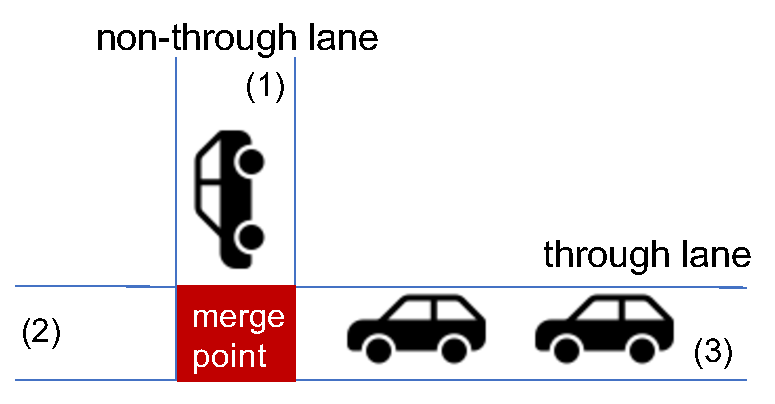
\includegraphics{Pictures/merge_point.pdf}}
\end{center}
\caption{Merge point}
\label{mergePoint_fig}
\end{figure}

To resolve the problem mentioned above, 
S. Aoki and R. Rajkumar~\cite{10.1145/3055004.3055028} have proposed the protocol called merging protocol.
%to prevent the collision in the merge point.
The protocol has two versions corresponding to two traffic environments: (1) only self-driving vehicles on the traffic (homogeneous traffic), 
(2) self-driving vehicles and human-driven vehicles on the traffic (heterogeneous traffic).
In the present paper, we mainly concentrate on the first version (1). 
The protocol requires each self-driving vehicle equiped with several necessary software systems such as navigation system or hardware devices such as sensors.
%These equipments are required since the self-driving vehicle get the necessary information for  vehicle systems such as lane information.
Further more, the authors also assumes each vehicle is able to uses some technologies such as WAVE \cite{4346439,5888501}, GPS to communication with other vehicles.
%Please refer to the paper~\cite{10.1145/3055004.3055028} for details.
%This protocol is designed for fully self-driving vehicle system which all the self-driving vehicle has a map database, A navigation system, an autonomous vehicle controller, a wireless communication interface, and a localization capability. 
%Map database and navigation can recognize which lane the vehicle in. Autonomous vehicle controller is used to actuate the self-driving vehicle traverse the chosen path. 
%The wireless interface is used to allow vehicles to send or receive messages. 
%It also use some perception system like LIDAR or camera~\cite{6629559} to avoid some unexpected crashing situations. 

%For fully self-driving vehicles crossing the merge point safely and efficiently, three priority states be designed: (i) Fully-priority state; (ii) Semi-priority state; and (iii) Fair state. 
All vehicles participating in the protocol are controlled based on three system states: fully-prioritized state, semi-prioritized state, and fair state. 
When the system is in a state, it can be changed to another state (e.g., from fully-prioritized state change to semi-prioritized state) by some trigger actions.
Each of them is explained in the upcoming sub-sections.

\subsection{Fully-prioritized state}
When the system is in a fully-prioritized state, vehicles running on the non-through lane cannot intervene those running on the through lane. 
It means that a non-through lane vehicle is allowed to enter the merge point only if no vehicle on the through lane is approaching the merge point.
Precisely, there are two cases that allow the non-through lane vehicle to do so:
\begin{itemize}
    \item all vehicles running on the through lane are far away from the merge point or there is no vehicle on the through lane, or
    \item two lanes have vehicles approaching the merge point, the vehicle on the non-through lane stops right before the merge point and waits until all through lane vehicles approaching the merge point crossed the merge point. 
\end{itemize}


% \begin{figure}[h]
% \begin{center}
% \scalebox{0.33}{\includegraphics{Pictures/fullyPrioritized.pdf}}
% \end{center}
% \caption{Fully-prioritized state}
% \label{fullyPri_fig}
% \end{figure}


\subsection{Semi-prioritized state}
\label{semi-case}
When the system is in a semi-prioritized state, a non-through lane vehicle has a chance to enter the merge point even though there exists some through lane vehicles approaching the merge point. 
%This state gives a vehicle running on the non-through lane permission to intervene the vehicle running on the through lane, if it finds there exists enough space between two through lane vehicles. 
If there exists enough space between two through lane vehicles approaching the merge point, a non-through lane vehicle approaching the merge point can use that space to enter the intersection.
%Semi-prioritized state gives vehicle a chance to enter the merge point although some through lane vehicles is approaching the merge point. If non-through lane vehicle detects it has enough space between two through lane vehicles which approaching the merge point, it will use the space to enter the merge point. 

% \begin{figure}[h]
% \begin{center}
% \scalebox{0.33}{\includegraphics{Pictures/semiPrioritizedNonthrough.pdf}}
% \end{center}
% \caption{Fully-prioritized state}
% \label{semiPriNT}
% \end{figure}

\subsection{Fair state}
The state of the system changes to a fair state if the traffic of the through lane is congested. 
In this state, through lane vehicles and non-though lane vehicles are allowed to enter the merge point alternately.
%In case the through lane is congested, the protocol moves to fair state.
%The state allows the vehicles on both lane enter the merge point alternately.
%If non-though lane vehicle find through lane is congested, the whole self-driving control system will move to Fair state.
%This state allows non-through lane vehicle and through lane vehicle enter the merge point alternately like a zipped merge.

% \begin{figure}[t]
% \begin{center}
% \scalebox{0.33}{\includegraphics{Pictures/fairState.pdf}}
% \end{center}
% \caption{Fair state}
% \label{semiPriNT}
% \end{figure}




% Algorithm 1, Algorithm 2 and Algorithm 3 present the algorithm of \textit{Autonomous Vehicle Protocol for Merge Points}. Algorithm 1 presents the protocol for the vehicle on the non-through lane, and Algorithm 2 presents the protocol for the vehicle on the through lane. In addition, Algorithm 3 presents the protocol for the vehicle on the non-through lane when the vehicle is in Fair state. The vehicles on the non-through lane, originally having the lower priority which are represented by $\omega_{l1}$, .. $\omega_{ln}$. The vehicles on the through lane originally having higher priority are denoted as $\omega_{h1}$, ... $\omega_{hn}$. The sequential subscript numbers indicate the vehicle order, meaning $\omega_{l1}$ is the leader vehicle on the non-through lane before the merge intersection.



% The CROSS message is not used in any algorithms because this perception is sufficiently safe for the intersection. However, it is used in order to enhance the reliability and safety of the protocol.


% \begin{algorithm}[t]
% \caption{Protocol for Vehicle $\omega_{l1}$ on non-through lane} 
% \label{alg:nlane}
% \While{\textit{not started the maneuver}}
% {
% SM( $\omega_{l1}$) = \textbf{REQUEST};\newline
% \uIf{\textit{not halting before the merge point}}
% {
% \uIf{\textit{No vehicle before the merge point}}{Start the maneuver;}
% \uElseIf{\textup{RM($\omega_{l1}$) = \textbf{APPROVE}}}{Start the maneuver;}
% \Else{Slow down (for halting right before the merge point);}
% }
% \Else{
% Halting before the merge point($\upsilon_{\omega_{h1}}$ = 0);\newline
% \uIf{\textit{not halting before the merge point}}{Start the maneuver;}
% \uElseIf{\textup{RM($\omega_{l1}$) = \textbf{APPROVE}}}{Start the maneuver;}
% \uElseIf{Average\{$\upsilon_{\omega_{h1}}$,..$\upsilon_{\omega_{hn}}$\}  $<$ $\psi$}
% {SM($\omega_{h1}$) = \textbf{ENTER};\newline
% SM($\omega_{l2}$, ..$\omega_{ln}$) = \textbf{STATE TRANSITION};\newline
% $\omega_{h1}$  transits to \textit{Fair state};\newline
% Start the maneuver;
% }
% \Else{
% \textit{k} = arg max \textit{D\{$\omega_{hi}$\}};\newline
% SM($\omega_{hk}$) = \textbf{INTERRUPT};\newline
% \If{\textup{RM($\omega_{hk}$) = \textbf{YIELD}}}
% {
% \While{$s_{1}$ sec}
% {
% \If{\textup{RM($\omega_{h(k-1)}$ = \textbf{EXIT}}}{Start the maneuver;}
% }
% }
% }
% }
% }
% \end{algorithm}


% Some other notations used in these algorithms.
% \begin{itemize}
%     \item $\upsilon_{\omega_{hk}}$: Current speed of the vehicle $\omega_{hk}$
%     \item $\psi$: Speed threshold
%     \item $s_{1}$: Time threshold for packet loss (for \textbf{INTERRUPT} or \textbf{YIELD})
%     \item $s_{2}$: Time threshold for packet loss (for \textbf{EXIT)}
%     \item $\Delta$: Time threshold for \textbf{ABOUT TO EXIT}
% \end{itemize}


% \begin{algorithm}[t]
% \caption{Protocol for Vehicle $\omega_{h1}$ on through lane}
% \label{alg:tlane}
% \uIf{RM($\omega_{h1}$) = \textbf{\textup{REQUEST}}}
% {
% \uIf{CollisionDetect($\omega_{h1}$, $\omega_{l1}$) = true}
% {SM($\omega_{l1}$) = \textbf{DECLINE};\newline Start the maneuver;}
% \Else{SM($\omega_{l1}$) = \textbf{APPROVE};\newline Start the maneuver;}
% }
% \uElseIf{RM($\omega_{h1}$) = \textbf{\textup{ENTER}}}
% {
% \While{$s_2$sec}
% {
% \uIf{RM($\omega_{l1}$) = \textbf{\textup{ABOUT TO EXIT}}}{
% SM($\omega_{l1}$) = \textbf{ENTER};\newline
% Going to start the maneuver;\newline
% \uIf{RM($\omega_{l1}$) $\neq$ \textbf{\textup{EXIT}} in $\Delta$sec later after \textbf{\textup{ABOUT TO EXIT}}}{Slow down and Halting;}
% \Else{Start the maneuver;}
% }
% \uElseIf{RM($\omega_{l1}$) = \textbf{\textup{EXIT}}}{Start the maneuver;}
% \Else{Halting;}
% }
% \uIf{No vehicle before the merge point}{Start the maneuver;}
% \Else{Halting;}
% }
% \uElseIf{RM($\omega_{l1}$) = \textbf{\textup{INTERRUPT}}}{\uIf{CollisionDetect($\omega_{h1}$, $\omega_{l1}$) = true}{Slow down(to make space for $\omega_{l1}$);\newline
% SM($\omega_{l1}$) = \textbf{YIELD};}
% \Else{SM($\omega_{l1}$) = \textbf{YIELD};}}
% \Else{Start the maneuver;}
% \end{algorithm}

% \begin{algorithm}[t]
% \caption{Protocol for Vehicle $\omega_{l1}$ in Fair state}
% \label{alg:fair}
% \uIf{right before the merge point}{
% \uIf{RM($\omega_{h1}$) = \textbf{\textup{ABOUT TO EXIT}}}{
% SM($\omega_{h2}$) = \textbf{ENTER};\newline
% SM($\omega_{l2}$, ..$\omega_{ln}$) = \textbf{STATE TRANSITION};\newline
% Going to start the maneuver;\newline
% \uIf{RM($\omega_{h1}$) $\neq$ \textbf{\textup{EXIT}} in $\Delta$sec later after \textbf{\textup{ABOUT TO EXIT}}}{Halting;}
% \Else{Start the maneuver;}
% }
% \uElseIf{RM($\omega_{h1}$) = \textbf{\textup{EXIT}}}{
% SM($\omega_{h2}$) = \textbf{ENTER};\newline
% SM($\omega_{l2}$, ..$\omega_{ln}$) = \textbf{STATE TRANSITION};\newline
% Start the maneuver;
% }
% \Else{Halting;}
% }
% \Else{Follow the vehicle in front;}
% \end{algorithm}

% In the \textit{Autonomous Vehicle Protocol for Merge Points}, three functions implies three priority state of non-through lane vehicles. (i)High throughput function; (ii) Intervention function; (iii) Zipper merge function. 


\section{Abstract Merging Protocol for Self-Driving Vehicles}
 \label{sect_reviproto}
% TODO: your abstract verion do nothing to resolve/mitigate the disadvantage problems mentioned here.  
%A merging protocol uses V2V communication and allows the self-driving vehicles merge into one lane from two different lanes. 
%Sending and receiving messages basing on network may not fully reliable because some data may lost during the transmission. 
%If one vehicle lose some messages sent by other vehicles, a serious collision may happen. 
%Furthermore, to make it more abstract, some information, such as vehicle speed, position on road, are ignored.
Based on the \textit{merging} protocol described in the last section, we abstract some parts to make another version namely abstract merging protocol (\textit{a-merging} protocol).
Our target is to conduct model checking to check that whether the protocol enjoy some desired properties such as mutual exclusion property (i.e., there is at most one vehicle crossing the merge point at any given time).
We use two separate queues to manage the vehicles on two lanes.
Each vehicle is attached with one of six statuses: \textit{running}, \textit{approaching}, \textit{stopped}, \textit{crossing}, \textit{crossed}, \textit{halting}.
The meaning of these statuses will be clear later on.
%Therefore, basing on the \textit{merging protocol}, we designed a abstract version of the protocol called \textit{abstract merging protocol (a-merging protocol)}.

%Therefore, basing on \textit{Autonomous Vehicle Protocol for Merge Points}, we designed a new protocol called \textit{Revised Autonomous Vehicle Protocol for Merge Points} .

%Basing on the \textit{Autonomous Vehicle Protocol for Merge Points}, we find 
In \textit{a-merging} protocol, there are three cases in which a non-through lane vehicle is allowed to enter the merge point: 
(i) no vehicle on through lane is approaching the merge point; 
(ii) some vehicles on the through lane are approaching the merge point but it has enough space between them; 
(iii) through lane and non-through lane vehicle enter the merge point alternately. 

Fig.~\ref{throughLaneStatus} graphically visualizes the transition of a through lane vehicle's status.
%Let us consider the status of vehicle on through lane shown in Fig.~\ref{throughLaneStatus} which has five statues. 
Each arrow represents the change of vehicle's status from one value to another value if some conditions denoted by a number are satisfied.

\begin{figure}[h]
\begin{center}
\scalebox{0.4}{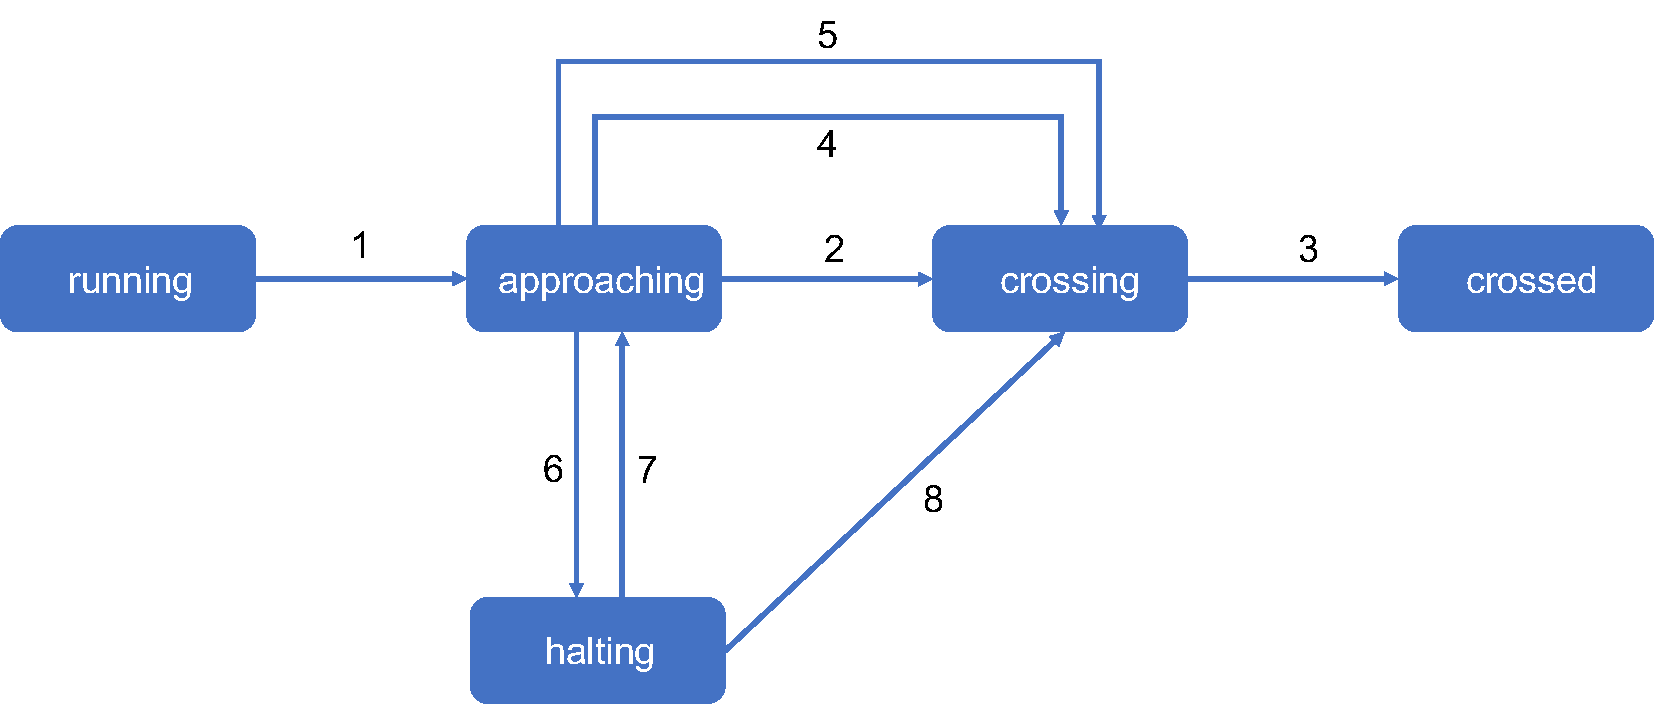
\includegraphics{Pictures/throughLane.pdf}}
\end{center}
\caption{Transition of a through lane vehicle's status}
\label{throughLaneStatus}
\end{figure}

Transitions are explained as follows:
\begin{enumerate}[]
    \item the vehicle is approaching the merge point. %1
    \item there is no vehicle crossing the merge point and the system is in a fully-prioritized state. %2
    \item the vehicle crossed the merge point. %3
    \item the through lane is congested (i.e., the number of vehicles running on the through lane greater than a specific number), and there is no vehicle crossing the merge point.  %4
    \item the system is in a fair state, and it is the through lane vehicle's turn, and there is no vehicle crossing the merge point. %5
    \item the  system is in a fair state and it is the non-through lane vehicle's turn. %6
    \item the  system is not in a fair state. %7
    \item the system is in a fair state, and it is the through lane vehicle's turn, and there is no vehicle crossing the merge point. %8
\end{enumerate}

Initially, each through lane vehicle has \textit{running} status, which mean that the vehicle is far away from the merge point.
The status of a vehicle change to \textit{approaching} from \textit{running} if the vehicle is approaching to the merge point.
If the system is not in a fair state, the vehicle's status change to \textit{crossing} from \textit{approaching} when there is no vehicle crossing merge point. 
Right after crossing the merge point, the status of it change to \textit{crossed}. 
From condition 4) to condition 8), the system falls into a fair state, the vehicle first check whether it is its turn or not. 
If it is the through lane's turn, vehicle changes its status from \textit{approaching} to \textit{crossing}. 
On the other hand, it changes its status to \textit{halting} from \textit{approaching}, and stops right before the merge point waiting until the through lane's turn.

Fig.~\ref{space} visualizes how a non-through lane vehicles can enter the merge point during a semi-prioritized state when there is a space between two vehicles running on the through lane. 
The blue circle represents the non-through lane vehicle, the red circle represents the through lane vehicles, and the white circle represents a space. 
Green area denotes the merge point.
Each vehicle or space is attached a different number.
%Figure \ref{space}.(a) shows that vehicle 1 on the non-through lane is approaching the merge point.
In the Fig.~\ref{space} (a), there are two through lane vehicles (i.e., \textcircled{2} and \textcircled{4}), and there is a space (i.e., \textcircled{3}) in the middle of the two vehicles that is enough to accommodate the third vehicle. 
The vehicles \textcircled{2} and \textcircled{4} are approaching the intersection.
According to the full-prioritized state, the vehicle \textcircled{1} needs to let the vehicles \textcircled{2} and \textcircled{4} cross the merge point first. 
Thus, as shown in Fig.~\ref{space} (b), the vehicle \textcircled{1} stops right before the merge point, while the vehicle \textcircled{2} passes through the intersection.
In Fig.~\ref{space} (c) and Fig.~\ref{space} (d), the vehicle \textcircled{1} enters the merge point because there exists a space on the through lane between \textcircled{2} and \textcircled{4}.
%Fig.~\ref{space} (c) and Fig.~\ref{space} (d) show the process of the vehicles on the non-through lane find that it has enough space to join the vehicles on the through lane and enter the merge point.

\begin{figure}[h]
	\begin{center}
		\scalebox{0.28}{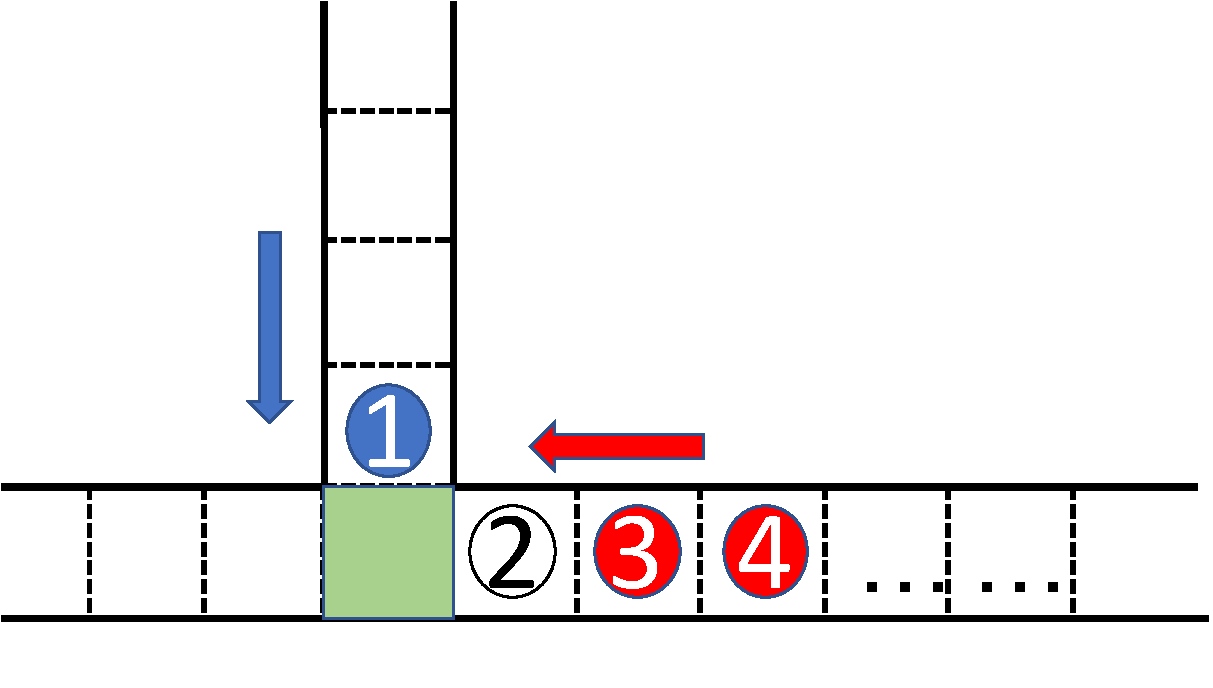
\includegraphics{Pictures/space.pdf}}
	\end{center}
	\caption{An example of semi-prioritized state}
	\label{space}
\end{figure}

\begin{figure}[h]
\begin{center}
\scalebox{0.36}{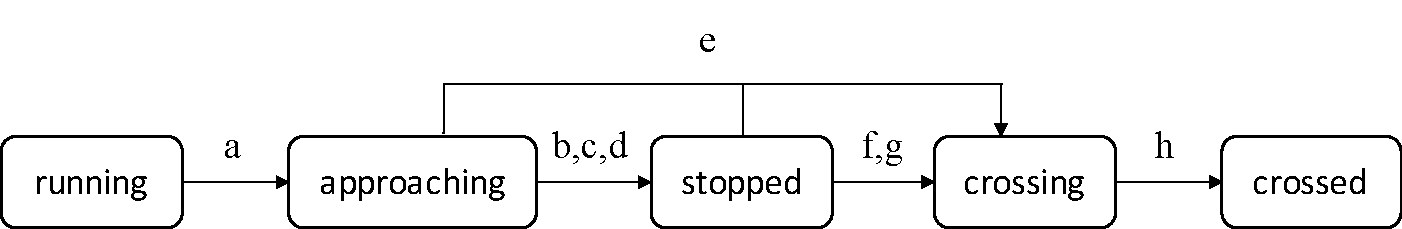
\includegraphics{Pictures/nonThroughLane.pdf}}
\end{center}
\caption{Transition of a non-through lane vehicle's status}
\label{nonThroughLaneStatus}
\end{figure}

Fig.~\ref{nonThroughLaneStatus} shows the transition of a non-through lane vehicle's status.
Transitions are explained as follows:
\begin{itemize}
    \item[a)] the vehicle is approaching the merge point. %1
    \item[b)] there exists a through lane vehicle that is approaching the merge point, and the system is not in a fair state. %2
    \item[c)] there is no vehicle on the through lane that is approaching the merge point, and the system is not in a fair state, and there is no vehicle crossing the merge point. %3
    \item[d)] the vehicle crossed the merge point. %4
    \item[e)] there is no vehicle on through lane that is approaching the merge point, and the system is not in a fair state, and there is no vehicle crossing the merge point. %5
    \item[f)] the system is in a semi-prioritized state, and there is no vehicle crossing the merge point. %6
    \item[g)] the system is in a fair state, and it is the non-through lane vehicle's turn, and there is no vehicle crossing the merge point. %7
    \item[h)] the system is in a fair state, and it is the through lane vehicle's turn. %8
    \item[i)] the system is not in a fair state. %9
    \item[j)] the system is in a fair state, and it is the through lane vehicle's turn. %10
    \item[k)] the system is in a fair state, and it is the non-through lane vehicle's turn, and there is no vehicle crossing the merge point. %11
    \item[l)] the system is in a fair state, and it is the non-through lane vehicle's turn, and there is no vehicle crossing the merge point. %12
\end{itemize}

Initially, all non-through lane vehicles receive \textit{running} as their statuses.
It changes to \textit{approaching} status when it approaches the merge point.
Let us consider the case when the system is in a fully-prioritized state first.
The non-through lane vehicle initially has lower priority than other vehicles running on the through lane.
Therefore, its status changes to \textit{stopped} from \textit{approaching} when there exists another through lane vehicle approaching to the merge point.
If there does not exist a vehicle running on the through lane with \textit{approaching} status, the vehicle changes its status to \textit{crossing} from \textit{stopped}.

The second case is when the system is in a fully-prioritized state.
If there exists a space between the merge point and another through lane vehicle whose status is \textit{approaching}, 
the vehicle changes its status to \textit{crossing} from \textit{stopped}.
%If vehicle on non-through lane finds no vehicle on through lane is approaching to the merge point, it will go to \textit{crossing} status from \textit{stopped} status. 
%If vehicle on non thorough lane find space before the merge point it knows Semi-prioritized state comes and it changes to \textit{crossing} status from \textit{stopped} status. After vehicle crossed the merge point, it moves to \textit{crossed} status.

When the system in a fair state, which is the last case.
%While vehicle on through lane changes to the Fair state, vehicle on non-through lane also moves to Fair state. 
If it is the through lane vehicle's turn, the vehicle's status changes to \textit{halting} from \textit{approaching} or \textit{stopped}. 
On the other hand, it changes the status to \textit{crossing} from \textit{approaching}, \textit{stopped} or \textit{halting}. 
 


 
\section{Formal Specification}
 \label{sect_formal}
%In the semi-prioritized state of the merging protocol, if there exists an enough space on through lane, a non-through lane vehicle can enter to the merge point.
We use two queues to maintain the vehicles running on the through lane and non-through lane, respectively.
Each element of the queue can be not only a vehicle, but also a space.
 %From the \textit{Revised Autonomous Vehicle Protocol for Merge Points }, we know that in the Semi-priority state, a space can accommodate a car, so we can divide the road into many small squares, and each small square can accommodate a car or a space or nothing.
%Furthermore, we use a global variable that contains 5 
%  (\verb!v![$vid$] : $lid$\verb!,!$vstat$\verb!,!$t$\verb!,!$lt$)
In this paper, a state is expressed as a soup of observable components.
To formalize the protocol, we use four observable components as follows:
\begin{itemize}
    \item (\verb!v[!$id$\verb!]:!$position$\verb!,!$vstat$) - $id$ is an ID (a nature number) of a vehicle or a space, $position$ is the lane that the vehicle or the space $id$ is located (either through lane or non-through lane), $vstate$ is the status of the vehicle if it is a vehicle. Initially, $vstate$ is \verb!space! if it is a space, or \verb!running! if it is a vehicle.
    \item (\verb!lane[!$position$\verb!]:!$q$) - $position$ is the through lane or non-through lane, and $q$ is a queue of vehicles and spaces. Initially, $q$ is \verb!empq!, which denotes an empty queue.
    \item (\verb!switch:!$c$\verb!,!$semi$\verb!,!$fair$\verb!,!$nonthrough$\verb!,!$nthrough$) - $c$ receives one of the following two values: \verb!noVehicleCrossing! indicating there is not any vehicle crossing the merge point, or \verb!vehicleCrossing! indicating there exists a vehicle crossing the merge point.
    $semi$ receives one of the following two values: \verb!semiPrioritized! indicating the system is in a semi-prioritized state, or \verb!noSemiPrioritized! indicating the system is in a fully-prioritized state. 
    $fair$ receives one of the following three values: \verb!noFair! indicating the system is not in a fair state, or \verb!fairT! indicating the system is in a fair state and it is the through lane vehicle's turn, or \verb!fairN! indicating the system is in a fair state and it is the non-through lane vehicle's turn.
    $nonthrough$ receives one of the following two values: \verb!noVeInNTLane! indicating there is not any non-through lane vehicle approaching the merge point, or \verb!veInNTLane! indicating there exists a non-through lane vehicle approaching the merge point. 
    $nthrough$ is the total number of through lane vehicles approaching the merge point.
    Initially, $c$, $semi$,$fair$,$nonthrough$ and $nthrough$ are \verb!noVehicleCrossing!, \verb!noSemiPrioritized!, \verb!noFair!, \verb!noVeInNTLane! and \verb!0!, respectively.
    \item (\verb!gstat! : $gstat$) -  $gstat$ is either \verb!fin! or \verb!nFin!.
	When it is \verb!fin!, all vehicles concerned have crossed the intersection.
\end{itemize}

We use 25 rewrite rules to define the transitions of the protocol.
%Let us consider a case such that the vehicle approaches the merge point, the status of the vehicle changes from the \verb!running! status to the \verb!approaching! status. 
%This case corresponds to condition 1 of two lanes.
%We use four rules to specify this case in which
%We use four rules to specify this process. 
%two rules for the through lane and two rules for the non-through lane.
The following two rules are defined to specify a set of transitions that
change a vehicle status from \verb!running! to \verb!approaching!, one for through lane vehicles, and another for non-through lane vehicles: 

\begin{small}
\begin{verbatim}
crl [approach_T] : {(gstat: nFin) 
(switch: B1,B2,B3,B4,numOfVeInTLane) 
(lane[L]: VS) (v[VI]: L,running) OCs} 
=> {(gstat: nFin) 
(switch: B1,B2,B3,B4,(numOfVeInTLane + 1)) 
(lane[L]: (VS ; VI)) (v[VI]: L,approaching) 
OCs} if L == Through .
\end{verbatim}
\end{small}
\begin{small}
\begin{verbatim}
crl [approach_N] : {(gstat: nFin) 
(switch: B1,B2,B3,B4,numOfVeInTLane) 
(lane[L]: VS) (v[VI]: L,running) OCs} 
=> {(gstat: nFin) 
(switch: B1,B2,B3,veInNTLane,numOfVeInTLane) 
(lane[L]: (VS ; VI)) (v[VI]: L,approaching) 
OCs} if L == Nothrough .
\end{verbatim}
\end{small}

\noindent 
where \verb!B1!, \verb!B2!, \verb!B3!, \verb!B4!, and \verb!B5! are Maude variables of sort \verb!Swich!, receiving the values \verb!noVehicleCrossing! or \verb!vehicleCrossing!, \verb!semiPrioritized! or \verb!noSemiPrioritized!, \verb!noFair! or \verb!fairT! or \verb!fairN!, \verb!noVeInNTLane! or \verb!veInNTLane!, respectively.
\verb!VI! and \verb!VI'! are Maude variable of natural numbers, denoting arbitrary vehicle IDs. 
\verb!VS! is a Maude variable of queues, possibly empty.
\_;\_ is the constructor of queues, where an underscore \_ is
a place holder where an argument (e.g., vehicle ID) is put. 
The first rewrite rule says that when the through lane has a vehicle whose status is \verb!running!, the status is changed to \verb!approaching!, the vehicle is enqueue into the queue of the through lane, and the value of the last component of \verb!swich! (\verb!numOfVeInTLane!) is increment.
%It means that \textit{(q1 ; q2) ; q3 = q1 ; (q2 ; q3)}. 
%\verb!empq! represents the queue is empty. 
%\verb!(numOfVeInTLane)! in the \verb!switch! means the length of queue on through lane (only count vehicle).
%%From \verb![approach_T1]! and \verb![approach_T2]! rules, \verb!(numOfVeInTLane + 1)! in the \verb!switch! means the size of queue which represent vehicle on through lane add 1. 
%\verb!VeInNTLane! in the \verb!switch! means the queue of the non-through lane is not empty. 
%Notice, vehicles whose status are \verb!running! cannot be counted in the queue (both lanes).
%
%We use the following states to express conditions of both lanes mentioned in~\ref{sect_reviproto} as follows:


The remaining rewrite rules are divided into four groups: a vehicle tries to enter the merge point when the system is in a fully-prioritized state; a vehicle tries to enter the merge point when the system is in a semi-prioritized state; a vehicle leaves the merge point when the system is in a fully-prioritized or semi-prioritized state;
when the system is in a fair state.
	
\begin{figure*}[tb]
\begin{center}
\scalebox{0.35}{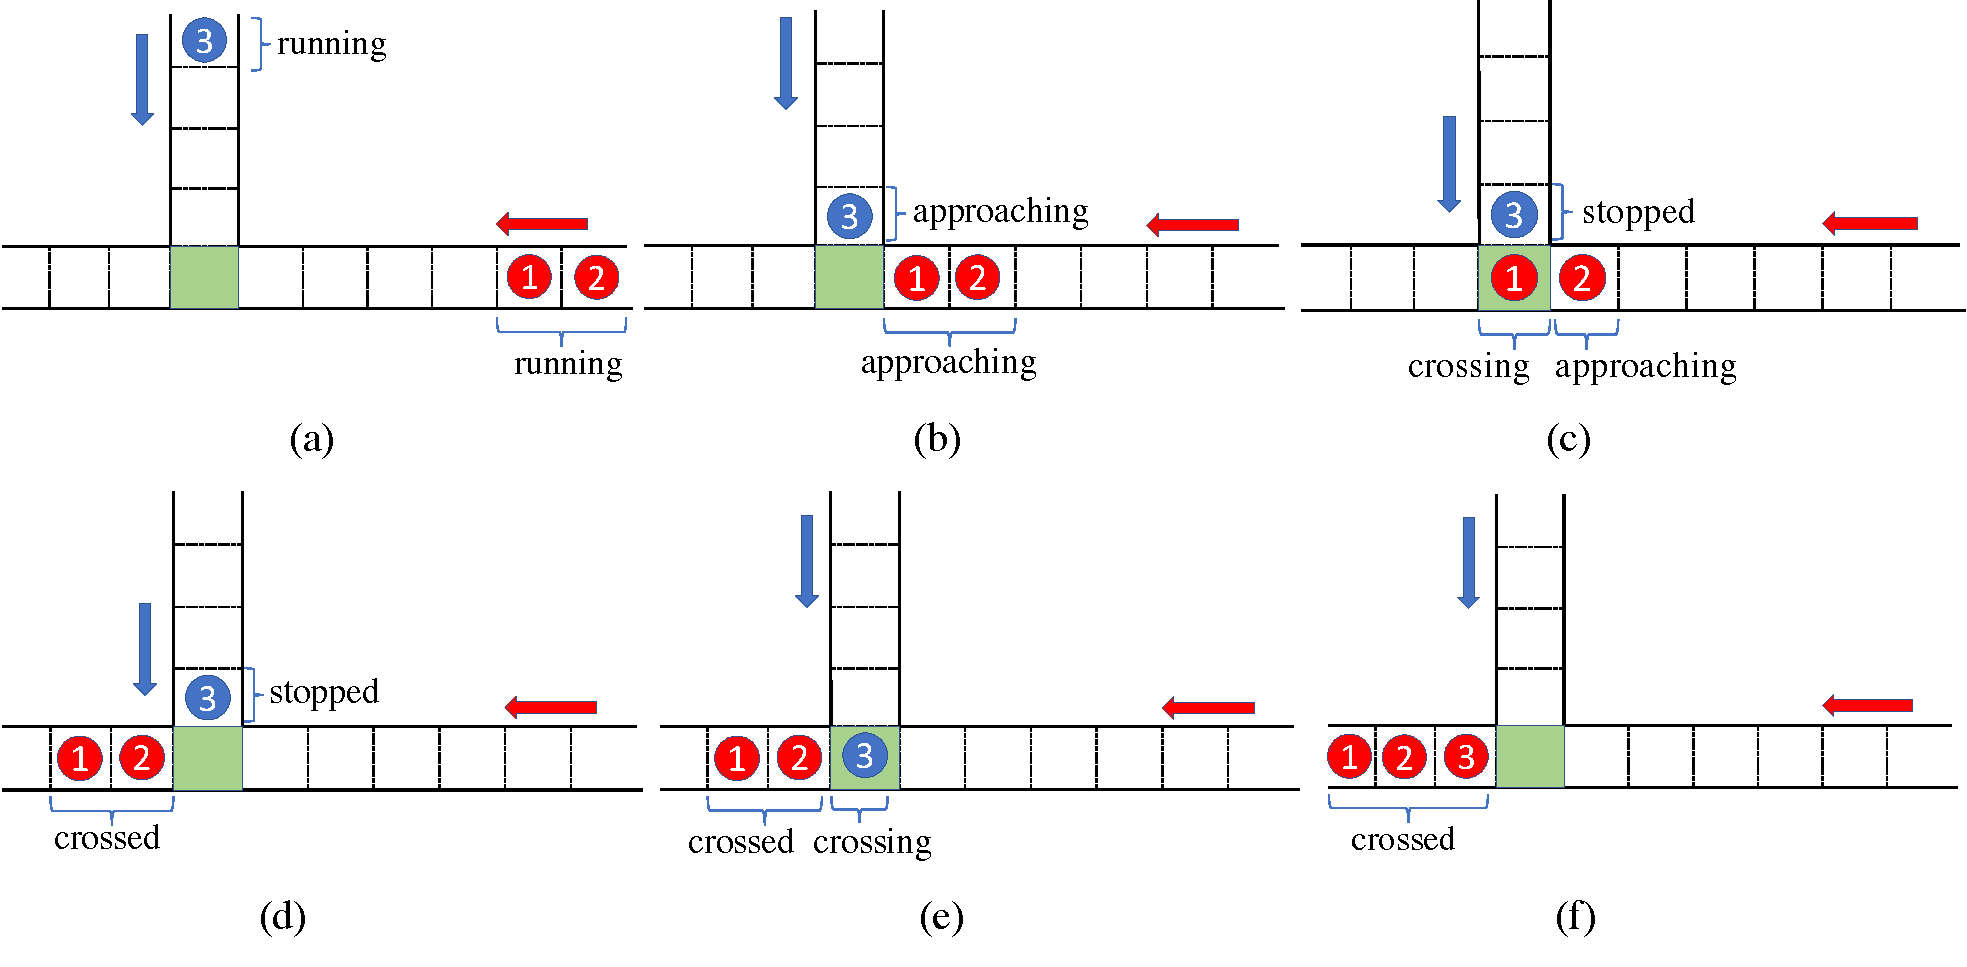
\includegraphics{Pictures/fullySim.pdf}}
\end{center}
\caption{An example of fully-prioritized state}
\label{fully_fig}
\end{figure*}

\subsection{A vehicle tries to enter the merge point when the system is in a fully-prioritized state}

Let us consider a concrete fully-prioritized state in which there are two through lane vehicles and one vehicle running on the non-through lane as shown in Fig.~\ref{fully_fig}. 
The initial state shown in Fig.~\ref{fully_fig} (a) is expressed as follows:
%Initially, the through lane and non-through lane both have one vehicle running on them. Here, the initial state is expressed as follows:
 
\begin{small}
\begin{verbatim}
{(gstat: nFin) (lane[Through]: empq) 
(lane[Nothrough]: empq) 
(v[1]: Through,running) 
(v[2]: Through,running)
(v[3]: Nothrough,running)
(switch: noVehicleCrossing,noSemiPrioritized,
noFair,noVeInNTLane,0)} .
\end{verbatim}
\end{small}

%\noindent \verb!v[1]! and \verb!v[2]! observable components represent two vehicles. 
%One of them is running on the through lane, the other one is running on the non-through lane. The observable component of \verb!switch! means no vehicle is crossing the merge point and the whole self-driving system is either in Semi-prioritized state or Fair state. \verb!noVeInNTLane! and \verb!0! show the queue of two lanes are empty.

Three rewrite rules are introduced in this case.
The first one \verb!full_T_crossing! specifies the set of transitions 2) explained in the previous section.
That is a through lane vehicle is allowed to pass the merge point is there is no vehicle crossing the merge point and the system is in a fully-prioritized state.
Fig.~\ref{fully_fig} (b) and (c) graphically visualize this kind of transition.
The rewrite rule is defined as follows:
%Condition 2 of the through lane is shown by rule \verb![full_T_crossing]!:

\begin{small}
\begin{verbatim}
crl [full_T_crossing] : {(gstat: nFin) 
(switch: noVehicleCrossing,noSemiPrioritized,
noFair,B4,numOfVeInTLane) 
(lane[L]: (VI ; VS)) (v[VI]: L,approaching) 
OCs} 
=> {(gstat: nFin) 
(switch: vehicleCrossing,noSemiPrioritized,
noFair,B4,numOfVeInTLane) 
(lane[L]: (VI ; VS)) (v[VI]: L,crossing) OCs} 
if L == Through .
\end{verbatim}
\end{small}


The second rewrite rule \verb!full_N_stop! specifies the set of transitions b) explained in the previous section.
That is a non-through lane vehicle which is approaching the merge point must stop right before the intersection if there exists a through lane vehicle that is approaching the merge point, and the system is not in a fair state. 
The rewrite rule is defined as follows:

\begin{small}
\begin{verbatim}
crl [full_N_stop] : {(gstat: nFin) 
(switch: B1,B2,noFair,B4,numOfVeInTLane) 
(lane[L]: (VI ; VS)) (v[VI]: L,approaching) 
OCs}
=> {(gstat: nFin)
(switch: B1,B2,noFair,B4,numOfVeInTLane) 
(lane[L]: (VI ; VS)) (v[VI]: L,stopped) OCs}
if L == Nothrough /\ numOfVeInTLane > 0 .
\end{verbatim}
\end{small}

The third rewrite rule \verb!full_N_crossing! specifies the set of transitions c) and e) explained in the previous section.
That is a non-through lane vehicle whose status is \verb!approaching! or \verb!stopped! is allowed to enter the merge point
if there is no vehicle on the through lane that is approaching the merge point, and the system is not in a fair state.
Fig.~\ref{fully_fig} (d) and (e) visualize this kind of transition.
The rewrite rule is defined as follows:

\begin{small}
\begin{verbatim}
crl [full_N_crossing] : {(gstat: nFin) 
(switch: noVehicleCrossing,noSemiPrioritized,
noFair,B4,0) 
(lane[L]: (VI ; VS)) (v[VI]: L,VeSt) OCs} 
=> {(gstat: nFin) 
(switch: vehicleCrossing,noSemiPrioritized,
noFair,B4,0) 
(lane[L]: (VI ; VS)) (v[VI]: L,crossing) OCs}
if L == Nothrough /\ 
(VeSt == approaching or VeSt == stopped) .
\end{verbatim}
\end{small}

\noindent
where \verb!VeSt! is Maude variable of sort \verb!VStat!, denoting arbitrary vehicle status.

\subsection{Semi-prioritized state}

%We proposed that observable component of (\verb!v[!$id$\verb!]: !$position$\verb!,!$vstat$) is a vehicle or space. 
%As mentioned in section~\ref{semi-case}, when the system is in a semi-prioritized state, a space appears in through lane.
%If it is a space on the non-through lane, we delete it because non-through lane initially has lower priority than the through lane.
%We use the following rule to specify this situation in Maude.
%
%\begin{footnotesize}
%\begin{verbatim}
%crl [semi_N_space2] : 
%{(gstat: nFin) 
%(switch: B1,B2,B3,B4,B5) 
%(lane[L]: (VI ; VS)) (v[VI']: L,space) OCs} 
%=> {(gstat: nFin) 
%(switch: B1,B2,B3,B4,B5) 
%(lane[L]: (VI ; VS)) OCs} 
%if L == Nothrough .
%\end{verbatim}
%\end{footnotesize}

%\noindent On the other side, If it is the space on the through lane, we push the space into the queue of the through lane.
When the system is in a semi-prioritized state, and there exists a space on the through lane, we push the space into the queue of the through lane.

\begin{small}
\begin{verbatim}
crl [semi_T_space] :
{(gstat: nFin) 
(switch: B1,B2,noFair,B4,numOfVeInTLane) 
(lane[L]: VS) (v[VI]: L,space) OCs}
=> {(gstat: nFin) 
(switch: B1,B2,noFair,B4,numOfVeInTLane) 
(lane[L]: (VS ; VI)) (v[VI]: L,yield) OCs}
if L == Through .
\end{verbatim}
\end{small}

\noindent
The rewrite rule changes
the status of the vehicle from \verb!space! to \verb!yield!.

When the status of the top vehicle on the through lane's queue is \verb!yield!, the second component of the \verb!switch! observable component changes to \verb!semiPrioritized!, meaning that the system changes to a semi-prioritized state.
This is done by the following rewrite rule:
%\noindent When the number which represents yield status is the first element of the through lane's queue, we move the \verb!noSemiPrioritized! in the \verb!switch! to \verb!semiPrioritized!, so that the entire system moves to the Semi-Prioritized state.
%This condition is specified by following rule.

\begin{small}
\begin{verbatim}
crl [semi_T_yield1] : 
{(gstat: nFin) 
(switch: noVehicleCrossing,B2,noFair,
veInNTLane,numOfVeInTLane) 
(lane[L]: (VI ; VI' ; VS)) (v[VI]: L,yield) 
OCs} 
=> {(gstat: nFin) 
(switch: noVehicleCrossing,semiPrioritized,
noFair,veInNTLane,numOfVeInTLane) 
(lane[L]: (VI' ; VS)) OCs} 
if L == Through .
\end{verbatim}
\end{small}

The rewrite rule \verb!semi_N_crossing! specifies the set of transitions f) explained in the previous section.
That is a non-through lane vehicle whose status is \verb!stopped! is allowed to enter the merge point
if the system is in a semi-prioritized state, and there is no vehicle crossing the merge point. 
The rewrite rule is defined as follows:

\begin{small}
\begin{verbatim}
crl [semi_N_crossing] : 
{(gstat: nFin) 
(switch: noVehicleCrossing,semiPrioritized,
 noFair,veInNTLane,numOfVeInTLane) 
(lane[L]: (VI ; VS)) (v[VI]: L,stopped) OCs} 
=> {(gstat: nFin) 
(switch: vehicleCrossing,semiPrioritized,
 noFair,veInNTLane,numOfVeInTLane) 
(lane[L]: (VI ; VS)) (v[VI]: L,crossing) OCs}
if L == Nothrough .
\end{verbatim}
\end{small}

There are some more rewrite rules to completely define the set of transitions in this case.
All of them can be found in the webpage shown in the Sect.~\ref{sect_intro}.

\subsection{A vehicle leaves the merge point when the system is in a fully-prioritized or semi-prioritized state}
%Then, let us consider vehicles' leaving of two lanes in fully-prioritized state and semi-prioritized state. 
%Firstly, no matter which vehicle crossed, the whole system should return to fully-prioritized state. 
%Firstly, the whole system returns to fully-prioritized if a vehicle has just crossed to the merge point.
%Secondly, we remove one vehicle out of the queue when it crossed and update the number of vehicle on the through lane.
%In non-through lane, \verb!veInNTLane! is changed to \verb!noVeInNTLane! if the last vehicle on non-through lane crossed the merge point.
%The followings rules refer to some cases of vehicle leaving on through lane and non-through lane.
%Secondly, we remove one vehicle out of the queue when it crossed, therefore, number of vehicle on the through lane should minus 1 and \verb!switch! should tell us whether ti is the last element in the queue of the non-through lane.
%Basing on these considerations, we specify vehicle leaving on through lane and non-through lane as follows:


%When a vehicle leaving the merge point, it is unqueue from the corresponding queue.

The following rewrite rule specifies a set of transitions when a through lane vehicle leaving the merge point:

\begin{small}
\begin{verbatim}
crl [T_leave] : {(gstat: nFin) 
(switch: vehicleCrossing,B2,noFair,B4,
numOfVeInTLane) (lane[L]: (VI ; VS)) 
(v[VI]: L,crossing) OCs} 
=> {(gstat: nFin) 
(switch: noVehicleCrossing,(if VS == empq 
then noSemiPrioritized else B2 fi),
noFair,B4,sd(numOfVeInTLane,1)) 
(lane[L]: VS) (v[VI]: !(L),crossed) OCs} 
if L == Through .
\end{verbatim}
\end{small}

\noindent
The rewrite rule says that when a through lane vehicle leaving the merge point, it is deleted from the queue of the through lane, the first component of observable component \verb!swich! is changed to \verb!noVehicleCrossing!, the last component of it is decrement (i.e., the number of through lane vehicles is decrement), and the second component of it is set to \verb!noSemiPrioritized! (i.e., the system state changes to fully-prioritized) if the queue becomes empty.

The following rewrite rule specifies a set of transitions when a non-through lane vehicle leaving the merge point:

\begin{small}
\begin{verbatim}
crl [N_leave] : {(gstat: nFin) 
(switch: vehicleCrossing,B2,noFair,
veInNTLane,numOfVeInTLane) 
(lane[L]: (VI ; VS)) (v[VI]: L,crossing) OCs} 
=> {(gstat: nFin) 
(switch: noVehicleCrossing,noSemiPrioritized,
noFair, (if VS == empq then noVeInNTLane 
else veInNTLane fi),numOfVeInTLane) 
(lane[L]: VS) (v[VI]: Through,crossed) OCs} 
if L == Nothrough .
\end{verbatim}
\end{small}

\noindent
The rewrite rule says that when a non-through lane vehicle leaving the merge point, it is deleted from the queue of the non-through lane, the first component of observable component \verb!swich! is changed to \verb!noVehicleCrossing!, the second component of it is set to \verb!noSemiPrioritized! (i.e., the system state changes to fully-prioritized), and the third component of it is set to \verb!noVeInNTLane! (i.e., there is not any vehicle on the non-through lane) if the queue becomes empty.

%\noindent Rule \verb![T_leave1]! shows vehicle on through lane leaving in fully-prioritized state and semi-prioritized state while rule \verb![N_leave2]! shows non-through lane.
%\noindent Rule \verb![T_leave1]! can be applied for the vehicle on through lane leaving in fully-prioritized state and semi-prioritized state; while rule \verb![N_leave2]! for the vehicle on non-through lane as shown in Fig.~\ref{fully_fig} (e) and (f).


\subsection{The system is in a fair state}
The system changes to a fair state if the traffic is congested, that is when the total number of vehicles running on the through lane is greater than some specific value.
The following rewrite rule specifies this kind of transitions:

%In the present paper, we take 3 as that specific value.
%
%It refers that if there exist vehicles on both lanes and at least three vehicles on through lane, the system moves to fair state.
%The situation refers to condition 5 of through lane and specified as following rule.

%The whole system moves to Fair state following the condition 5 of through lane. 
%In our formal specification, we set the explicit number as 3. 
%showing as follows:

\begin{small}
\begin{verbatim}
crl [fair_T_first_crossing] : 
{(gstat: nFin) 
(switch: noVehicleCrossing,B2,
noFair,veInNTLane,numOfVeInTLane) 
(lane[L]: (VI ; VS)) (v[VI]: L,approaching) 
OCs} 
=> {(gstat: nFin) 
(switch: vehicleCrossing,B2,
fairT,veInNTLane,numOfVeInTLane) 
(lane[L]: (VI ; VS)) (v[VI]: L,crossing) OCs} 
if L == Through /\ numOfVeInTLane >= 3 .
\end{verbatim}
\end{small}

\noindent
The rewrite rule says that when the number of vehicles running on the through lane is greater than or equals to 3 (a specific value), the system changes to a fair state with the through lane's vehicle turn first, and concurrently the top vehicle on the through lane is allowed to enter the merge point.
%\noindent We not only use the third variable of \verb!switch! to show the Fair state, but also use it to control two lane's turn when it in fair state. 
%\verb!fairT! means it is through lane's turn while \verb!fairN! means non-through lane's turn. 
%The formal specification is shown as follows:

The rewrite rule \verb!fair_T_crossing! specifies the set of transitions 5) and 8) explained in the previous section.
That is when the system is in a fair state, it is the through lane vehicle's turn, and the status of top of the though lane queue is \verb!halting! or \verb!approaching!, its status will be changed to \verb!crossing!, meaning that it is allowed to cross the merge point.
The rewrite rule is defined as follows:

\begin{small}
\begin{verbatim}
crl [fair_T_crossing] : {(gstat: nFin)
(switch: noVehicleCrossing,B2,fairT,
veInNTLane,numOfVeInTLane)
(lane[L]: (VI ; VS)) (v[VI]: L,VeSt) OCs} 
=> {(gstat: nFin) 
(switch: vehicleCrossing,B2,fairT,
veInNTLane,numOfVeInTLane) 
(lane[L]: (VI ; VS)) (v[VI]: L,crossing) OCs} 
if L == Through /\ 
(VeSt == approaching or VeSt == halting) .
\end{verbatim}
\end{small}

The rewrite rule \verb!fair_N_crossing! specifies the set of transitions g), k), and l) explained in the previous section.
That is when the system is in a fair state, it is the non-through lane vehicle's turn, and the status of top of the non-though lane queue is \verb!halting! or \verb!approaching! or \verb!stopped!, its status will be changed to \verb!crossing!, meaning that it is allowed to cross the merge point.
The rewrite rule is defined as follows:

\begin{small}
	\begin{verbatim}
crl [fair_N_crossing] : {(gstat: nFin) 
(switch: noVehicleCrossing,B2,fairN,
veInNTLane,numOfVeInTLane) 
(lane[L]: (VI ; VS)) (v[VI]: L,VeSt) OCs} 
=> {(gstat: nFin) 
(switch: vehicleCrossing,B2,fairN,
veInNTLane,numOfVeInTLane) 
(lane[L]: (VI ; VS)) (v[VI]: L,crossing) OCs} 
if L == Nothrough /\ (VeSt == approaching 
or VeSt == stopped or VeSt == halting) .
\end{verbatim}
\end{small}

When a vehicle leaves the merge point, we not only need to remove it out of the queue, but also need to hand over the turn to the other lane, if it is not the last vehicle in queue.
On the other hand, if it is the last vehicle, we change the system back to a fully-priority state.
Two rewrite rules are introduced as follows:

\begin{small}
\begin{verbatim}
crl [fair_T_crossed] : {(gstat: nFin) 
(switch: vehicleCrossing,B2,fairT,B4,
numOfVeInTLane) (lane[L]: (VI ; VS)) 
(v[VI]: L,crossing) OCs} 
=> {(gstat: nFin) (switch: noVehicleCrossing,
(if VS == empq then noSemiPrioritized else B2 
fi), 
(if VS == empq then noFair else fairN fi), 
B4,sd(numOfVeInTLane,1)) 
(lane[L]: VS) (v[VI]: L,crossed) OCs} 
if L == Through .
\end{verbatim}
\end{small}

\begin{small}
	\begin{verbatim}
crl [fair_N_crossed] : {(gstat: nFin) 
(switch: vehicleCrossing,B2,fairN,B4,
numOfVeInTLane) (lane[L]: (VI ; VS)) 
(v[VI]: L,crossing) OCs} 
=> {(gstat: nFin) (switch: noVehicleCrossing,
(if VS == empq then noSemiPrioritized else B2 
fi), 
(if VS == empq then noFair else fairT fi), 
(if VS == empq then noVeInNTLane else B4 fi),
numOfVeInTLane) (lane[L]: VS) 
(v[VI]: L,crossed) OCs} 
if L == Nothrough .
\end{verbatim}
\end{small}

There are also some more rewrite rules to completely define the set of transitions when the system is in a fair state, but because of the page limitation, we cannot present all of them.
Those rewrite rules can be found in the webpage shown in the Sect.~\ref{sect_intro}.

%In Fair state, the traffic on the through lane is congested. 
%Therefore, we use \verb!switch! to protect space from approaching the merge point in our formal specification.
%However, there is a situation that space has already in the queue of the through lane when it in Fair state. 
%We delete the space when it comes to that situation to keep the order correctly. 
%If it is the last element in the queue of the through lane, we move the state back to the Fully-prioritized state.
%
%\begin{footnotesize}
%\begin{verbatim}
%crl [fair_space1] :
%{(gstat: nFin) (switch: B1,B2,
%fairT,B4,numOfVeInTLane) 
%(lane[L]: (VI ; VI' ; VS)) (v[VI]: L,yield) OCs} 
%=> {(gstat: nFin) (switch: B1,B2
%,fairT,B4,numOfVeInTLane) (lane[L]: VI' ; VS) OCs} 
%if L == Through .
%
%crl [fair_space2] : 
%{(gstat: nFin) (switch: B1,B2,
%fairT,B4,numOfVeInTLane) 
%(lane[L]: VI) (v[VI]: L,yield) OCs} 
%=> {(gstat: nFin) (switch: B1,B2,
%noFair,B4,numOfVeInTLane) (lane[L]: empq) OCs} 
%if L == Through .
%\end{verbatim}
%\end{footnotesize}
%
%\noindent Condition 7 in \textit{Revised Autonomous Vehicle Protocol for Merge Points} of through lane and condition 9 in \textit{Revised Autonomous Vehicle Protocol for Merge Points} of non-through lane mean vehicle in halting status should back to approaching status because halting status is the exclusive status of Fair state.
%We specify these two conditions as follow:
%
%\begin{footnotesize}
%\begin{verbatim}
%rl [fair_exit] : 
%{(gstat: nFin) (switch: B1,B2,
%noFair,B4,numOfVeInTLane) 
%(lane[L]: (VI ; VS)) (v[VI]: L,halting) OCs} 
%=> {(gstat: nFin) (switch: B1,B2,
%noFair,B4,numOfVeInTLane) (lane[L]: (VI ; VS)) 
%(v[VI]: L,approaching) OCs} .
%if L == Through .
%\end{verbatim}
%\end{footnotesize}










% In Figure \ref{fully_fig}.(a), if two vehicle is approaching the merge point, vehicle on non-through lane will stop before the merge point and let 


% \verb!veInNTLane! shows non-through lane has vehicle which is approaching the merge point and \verb!numOfVeInTLane! explains number of vehicle on through lane is approaching the merge point. 


 
\section{Model Checking}
\label{sect_model}
There are three desired properties the \textit{a-merging} protocol should enjoy:
\begin{itemize}
    \item \textit{Mutual exclusion} - There is at most one vehicle crossing the merge point at any given time.
    \item \textit{Deadlock freedom} - There is no deadlock state.
    \item \textit{Starvation freedom} - If a vehicle is trying to cross the merge point, then the vehicle must eventually pass the merge point.
\end{itemize}

%We need an initial state that can cover all three states in our \textit{Revised Autonomous Vehicle Protocol for Merge Points}.
%Therefore, we put two space and three vehicles on the through lane, one space and three vehicles on the non-through lane.
%To cover all situations (three states) in the \textit{a-merging} protocol, we assume that two spaces and three vehicles on the through lane, one space and three vehicles on the non-through lane.
%The \verb!init! is shown as follows:

For the three experiments checking that the protocol enjoys the three properties mentioned above, we use the same initial state in which there are six vehicles participating. The initial state namely\verb!init! is defined as follows:
\begin{small}
\begin{verbatim}
{(gstat: nFin) 
(lane[Through]: empq) (lane[Nothrough]: empq) 
(v[1]: Through,space) (v[3]: Nothrough,space)
(v[2]: Through,space) (v[4]: Through,running)
(v[5]: Through,running) 
(v[6]: Through,running)
(v[7]: Nothrough,running) 
(v[8]: Nothrough,running)
(v[9]: Nothrough,running)
(switch: noVehicleCrossing,noSemiPrioritized
noFair,noVeInNTLane,0)} .
\end{verbatim}
\end{small}

\noindent
Three vehicles run on the through lane, while three others arrive from the non-through lane.
Furthermore, we also assume that there exist three space locations.

\subsection{Mutual exclusion}

The \textit{mutual exclusion} property can be checked by the following search commmand:

\begin{small}
\begin{verbatim}
search [1] in MTAS15 : 
init =>* {(v[VI]: LN, crossing) 
(v[VI']: LT, crossing) OCs} 
            such that VI =/= VI' .
\end{verbatim}
\end{small}

\noindent
where \verb!MTAS15! is the specification of the \textit{a-merging} protocol.
The search commands tries to find a state from the initial state \verb!init! such that two vehicles are crossing the merge point.
After about 2 minutes, Maude finished without finding any such a state.
It confirms that when  there are six vehicles participating, the protocol enjoys the \textit{mutual exclusion} property.

\subsection{Deadlock freedom}
To check that there is no deadlock state, we use the following command:

\begin{small}
\begin{verbatim}
search [1] in MTAS15 : init =>! {OCs} .
\end{verbatim}
\end{small}

\noindent
%This command tries to find a state that cannot let all vehicles crossed the merge point. 
No state was found. The experiment finished after around 2 minutes.
%It does not find any such state.
%Therefore, our \textit{a-merging} protocol also enjoy the \textit{deadlock freedom} property for the \verb!init!.


\subsection{Starvation freedom}
To model check that the protocol enjoys the \textit{starvation freedom} property, we need to employ Maude LTL model checking facilities.
% define $P_{a-merging}$ and $L_{a-merging}$. 
%$P_{a-merging}$ consists of one atomic proposition \verb!Fin!.
%$L_{a-merging}$ is defined as follows:
We first define two atomic propositions namely \verb!want! and \verb!passed! which takes a vehicle IDs as their argument. 
They are defined via the following equations:

\begin{small}
\begin{verbatim}
eq {(v[VI]: L,approaching) OCs} |= 
  want(VI) = true .
eq {(v[VI]: L,crossed) OCs} |= 
  passed(VI) = true .
eq {OCs} |= PROP = false [owise] .
\end{verbatim}
\end{small}

\noindent
where \verb!PROP! is a Maude variable of atomic propositions, \verb!|=! is a Maude symbol for satisfaction relation in LTL,
%The two equations mean that for all states $s$ $\in$ $P_{a-merging}L_{a-merging}(s)$ = {\verb!Fin!} if and only if $s$ contains (\verb!gstat : fin!). 
\verb!owise! is the abbreviation of otherwise, indicating that this equation will only be applied if all of the previous equations above it cannot be applied. 
The equations say that \verb!want(VI)! holds in a state $s$ iff $s$ contains \verb!(v[VI]: L,approaching)!, which means that the vehicle \verb!VI! is trying to enter the merge point. 
Likewise, \verb!passed(VI)! holds in a state $s$ iff $s$ contains \verb!(v[VI]: L,crossed)!, which means that the vehicle \verb!VI! already passed the merge point. 

The \textit{starvation freedom} property for each vehicle is then defined by the LTL formula \verb!lofree0!  as follows:
%We also define two LTL formulas as follows:

\begin{small}
\begin{verbatim}
eq lofree0(VI) = (want(VI) |-> passed(VI)) .
\end{verbatim}
\end{small}

\noindent
The formula says that if a vehicle \verb!VI! trying to cross the merge point, it eventually will pass through the merge point.
After that, the complete \textit{starvation freedom} property is specified by the LTL formula \verb!lofree! as follows:

\begin{small}
\begin{verbatim}
eq lofree = lofree0(4) /\ lofree0(5) /\ 
				lofree0(6) /\ lofree0(7) /\ 
				lofree0(8) /\ lofree0(9).
\end{verbatim}
\end{small}

The following command is used to model check the property:
\begin{small}
\begin{verbatim}
red in MTAS15-CHECK : modelCheck(init,lofree) .
\end{verbatim}
\end{small}

\noindent
No counterexamples were found. It took about 2 minutes for Maude to complete the model checking. 
Consequently, we can conclude that the protocol enjoys the \textit{starvation freedom} property with six vehicles participating in the protocol.

%\noindent where \verb!<>! is the LTL eventually connective $\diamondsuit$.
%We run the Maude command \verb!modelCheck(init, halt)! to check whether the protocol enjoys the \textit{starvation freedom} property.
%The program returns no counterexample.
%Therefore, the \textit{a-merging} protocol enjoys the property for the \verb!init!.

 
 
\section{Related Work}
 \label{sect_Relate}
 
 An autonomous vehicle intersection control protocol called LJPL protocol has been proposed to handle the mutual exclusion property in the intersection~\cite{LimJongBeom2018Aedm}.
 The authors design two type of lanes: concurrent and conflict lanes. 
 The protocol allows that the vehicles on concurrent lanes can enter the intersection simultaneously while the vehicles on conflict lanes cannot enter the intersection simultaneously.
 The intersection in the LJPL protocol is applied to the traffic which containing eight lanes, while the \textit{merging} protocol or \textit{a-merging} protocol focuses on two lanes.
 M.N.Aung, et.al~\cite{DBLP:conf/seke/AungP019} has specified and model checked the LJPL protocol in Maude.
 They have revised the protocol to avoid the deadlock state that cannot decide the order of two vehicle on two conflict lanes have same time arrival.
 In our case, we also use Maude to model check some properties of our protocol.
  
 Vaio, et. al.~\cite{8790807} have proposed a protocol to handle the intersection which may contain 12 lanes.
 They define Conflicting Area (CA) where collisions could occur, and Cooperative Zone (CZ) where each vehicle is able to communicate with its neighbors. 
 The authors describe their problem into undirected graph where a node represents a vehicle and an edge represents a communication link between two vehicles.
 The experiment uses three autonomous vehicle to confirm their effective theoretical analysis.
 Currently, we do not find any other works to use formal methods for this work.
 One piece of our future is to specify this protocol and make it more reliable by formal methods.
 
 








\section{Conclusion}
\label{concl_sect}

We have proposed a protocol call \textit{a-merging} protocol based on the a merging protocol~\cite{10.1145/3055004.3055028}, formally specified and conducted some experiments by model checking in Maude.
%We have revised the \textit{Autonomous Vehicle Protocol for Merge Points} \cite{10.1145/3055004.3055028} and some case studies in our revised protocol and formal specified it in Maude.
%We also model checked our formal specification with Maude model checking facilities.
We have encountered the state explosion problem when we tried to put more vehicle running on two lanes to model check our abstract protocol enjoys some properties in other situations.
In the future, we need to use theorem proving, such as CafeOBJ~\cite{DiaconescuF98}, to prove our proposed protocol enjoys some desired properties in general.



% An example of a floating figure using the graphicx package.
% Note that \label must occur AFTER (or within) \caption.
% For figures, \caption should occur after the \includegraphics.
% Note that IEEEtran v1.7 and later has special internal code that
% is designed to preserve the operation of \label within \caption
% even when the captionsoff option is in effect. However, because
% of issues like this, it may be the safest practice to put all your
% \label just after \caption rather than within \caption{}.
%
% Reminder: the "draftcls" or "draftclsnofoot", not "draft", class
% option should be used if it is desired that the figures are to be
% displayed while in draft mode.
%
%\begin{figure}[!t]
%\centering
%\includegraphics[width=2.5in]{myfigure}
% where an .eps filename suffix will be assumed under latex, 
% and a .pdf suffix will be assumed for pdflatex; or what has been declared
% via \DeclareGraphicsExtensions.
%\caption{Simulation Results}
%\label{fig_sim}
%\end{figure}

% Note that IEEE typically puts floats only at the top, even when this
% results in a large percentage of a column being occupied by floats.


% An example of a double column floating figure using two subfigures.
% (The subfig.sty package must be loaded for this to work.)
% The subfigure \label commands are set within each subfloat command, the
% \label for the overall figure must come after \caption.
% \hfil must be used as a separator to get equal spacing.
% The subfigure.sty package works much the same way, except \subfigure is
% used instead of \subfloat.
%
%\begin{figure*}[!t]
%\centerline{\subfloat[Case I]\includegraphics[width=2.5in]{subfigcase1}%
%\label{fig_first_case}}
%\hfil
%\subfloat[Case II]{\includegraphics[width=2.5in]{subfigcase2}%
%\label{fig_second_case}}}
%\caption{Simulation results}
%\label{fig_sim}
%\end{figure*}
%
% Note that often IEEE papers with subfigures do not employ subfigure
% captions (using the optional argument to \subfloat), but instead will
% reference/describe all of them (a), (b), etc., within the main caption.


% An example of a floating table. Note that, for IEEE style tables, the 
% \caption command should come BEFORE the table. Table text will default to
% \footnotesize as IEEE normally uses this smaller font for tables.
% The \label must come after \caption as always.
%
%\begin{table}[!t]
%% increase table row spacing, adjust to taste
%\renewcommand{\arraystretch}{1.3}
% if using array.sty, it might be a good idea to tweak the value of
% \extrarowheight as needed to properly center the text within the cells
%\caption{An Example of a Table}
%\label{table_example}
%\centering
%% Some packages, such as MDW tools, offer better commands for making tables
%% than the plain LaTeX2e tabular which is used here.
%\begin{tabular}{|c||c|}
%\hline
%One & Two\\
%\hline
%Three & Four\\
%\hline
%\end{tabular}
%\end{table}


% Note that IEEE does not put floats in the very first column - or typically
% anywhere on the first page for that matter. Also, in-text middle ("here")
% positioning is not used. Most IEEE journals/conferences use top floats
% exclusively. Note that, LaTeX2e, unlike IEEE journals/conferences, places
% footnotes above bottom floats. This can be corrected via the \fnbelowfloat
% command of the stfloats package.


% conference papers do not normally have an appendix


% use section* for acknowledgement
% \section*{Acknowledgment}

% The authors would like to thank...
% more thanks here


% trigger a \newpage just before the given reference
% number - used to balance the columns on the last page
% adjust value as needed - may need to be readjusted if
% the document is modified later
% \IEEEtriggeratref{8}
% The "triggered" command can be changed if desired:
% \IEEEtriggercmd{\enlargethispage{-5in}}

% references section

% can use a bibliography generated by BibTeX as a .bbl file
% BibTeX documentation can be easily obtained at:
% http://www.ctan.org/tex-archive/biblio/bibtex/contrib/doc/
% The IEEEtran BibTeX style support page is at:
% http://www.michaelshell.org/tex/ieeetran/bibtex/
\bibliographystyle{IEEEtran} \bibliography{paper}
%\bibliographystyle{IEEEtran} \bibliography{IEEEabrv,paper}
% argument is your BibTeX string definitions and bibliography database(s)
%\bibliography{IEEEabrv,../bib/paper}
%
% <OR> manually copy in the resultant .bbl file
% set second argument of \begin to the number of references
% (used to reserve space for the reference number labels box)

% \begin{thebibliography}{1}
% 
% \bibitem{IEEEhowto:kopka}
% H.~Kopka and P.~W. Daly, \emph{A Guide to \LaTeX}, 3rd~ed.\hskip 1em plus
%   0.5em minus 0.4em\relax Harlow, England: Addison-Wesley, 1999.
% 
% \end{thebibliography}

% that's all folks
\end{document}
